\documentclass[a4paper,10pt]{article}
\usepackage[brazil]{babel}
\usepackage[utf8]{inputenc}
\usepackage[T1]{fontenc}
\usepackage{amsmath}
\usepackage{hyperref}
\usepackage{url}
\usepackage{graphicx}
\usepackage{subfigure}

    \usepackage{xcolor,listings}
    \usepackage{textcomp}
    \usepackage{color}

    \definecolor{codegreen}{rgb}{0,0.6,0}
    \definecolor{codegray}{rgb}{0.5,0.5,0.5}
    \definecolor{codepurple}{HTML}{C42043}
    \definecolor{backcolour}{HTML}{F2F2F2}
    \definecolor{bookColor}{cmyk}{0,0,0,0.90}  
    \color{bookColor}

    \lstset{upquote=true}

    \lstdefinestyle{mystyle}{
				language=SQL,
				deletekeywords={IDENTITY},
				deletekeywords={[2]INT},
				morekeywords={clustered},
				framesep=8pt,
				xleftmargin=40pt,
				tabsize=1,
				%framexleftmargin=40pt,
				frame=tb,
				framerule=0pt,
        backgroundcolor=\color{backcolour},   
        commentstyle=\color{codegreen},
        keywordstyle=\color{codepurple},
        numberstyle=\footnotesize\color{codegray},
        stringstyle=\color{codepurple},
        basicstyle=\footnotesize,
        breakatwhitespace=false,         
        breaklines=true,                 
        captionpos=b,                    
        keepspaces=true,                 
        numbers=left,                    
        numbersep=-10pt,                  
        showspaces=false,                
        showstringspaces=false,
        showtabs=false,      
    }
    \lstdefinestyle{cstyle}{
				language=c++,
				basicstyle=\ttfamily,
				keywordstyle=\color{blue}\ttfamily,
				stringstyle=\color{red}\ttfamily,
				commentstyle=\color{green}\ttfamily,
				morecomment=[l][\color{magenta}]{\#},
				tabsize=1,
				framesep=4pt,
				xleftmargin=20pt,
				%framexleftmargin=40pt,
				frame=tb,
				framerule=0pt,
        backgroundcolor=\color{backcolour},   
        %commentstyle=\color{codegreen},
        %keywordstyle=\color{codepurple},
        numberstyle=\footnotesize\color{codegray},
        %stringstyle=\color{codepurple},
        basicstyle=\footnotesize,
        breakatwhitespace=false,         
        breaklines=true,                 
        captionpos=b,                    
        keepspaces=true,                 
        numbers=none,                    
        numbersep=-10pt,                  
        showspaces=false,                
        showstringspaces=false,
        showtabs=false,      
    }		
		
    \lstset{style=mystyle} 

\title{Sistema de Cinema}
\author{
Felipe Luís Pinheiro - 18/0052667 \and 
João Pedro C.N. Mota - 17/0106144 \and 
Pedro Catelli - 17/0112624 \and
Pedro Oliveira - 17/0163768}

\begin{document}

\maketitle
%\makeindex

\begin{abstract}
Neste relatório desenvolvemos os requisitos básicos de um sistema de banco de dados para um modelo de vendas de ingresso de um cinema. 

Link para o repositório: \url{https://github.com/flpinheiro/banco_de_dados}.

O projeto do programa que usa esse sistema de banco de dados está no repositorio : \url{https://github.com/flpinheiro/UnBCineFlixMVC}
\end{abstract}

\section{Introdução}

Requisitos gerais:

\begin{itemize}
	\item Um cinema pode ter muitas salas, sendo necessário, por tanto, registrar informações a respeito de cada uma, como sua capacidade, ou seja, o numero de assentos disponíveis.
	\item O cinema apresenta muitos filmes. Um filme tem informações, titulo e duração. Assim, sempre que um filme for ser apresentado, deve-se registrá-lo também.
	\item Um mesmo filme pode ser apresentado em diferentes salas e em horários diferentes. Cada apresentação em uma determinada sala e horário é chamada sessão. Um filme sendo apresentado em uma sessão tem um conjunto máximo de ingressos, determinado pela capacidade da sala.
	\item Os clientes do cinema podem comprar ou não ingressos para assistir a uma sessão. O
funcionário deve intermediar a compra do ingresso. Um ingresso deve conter informação
como o tipo de ingresso (Meio ingresso ou ingresso inteiro). Além disso, um cliente só pode
comprar ingressos para sessões ainda não encerradas.
\end{itemize}

\section{Diagrama de Entidade Relacionamento}

Na figura \ref{fig:mer} mostramos a primeira versão conceitual do sistema do

\begin{figure}[h]
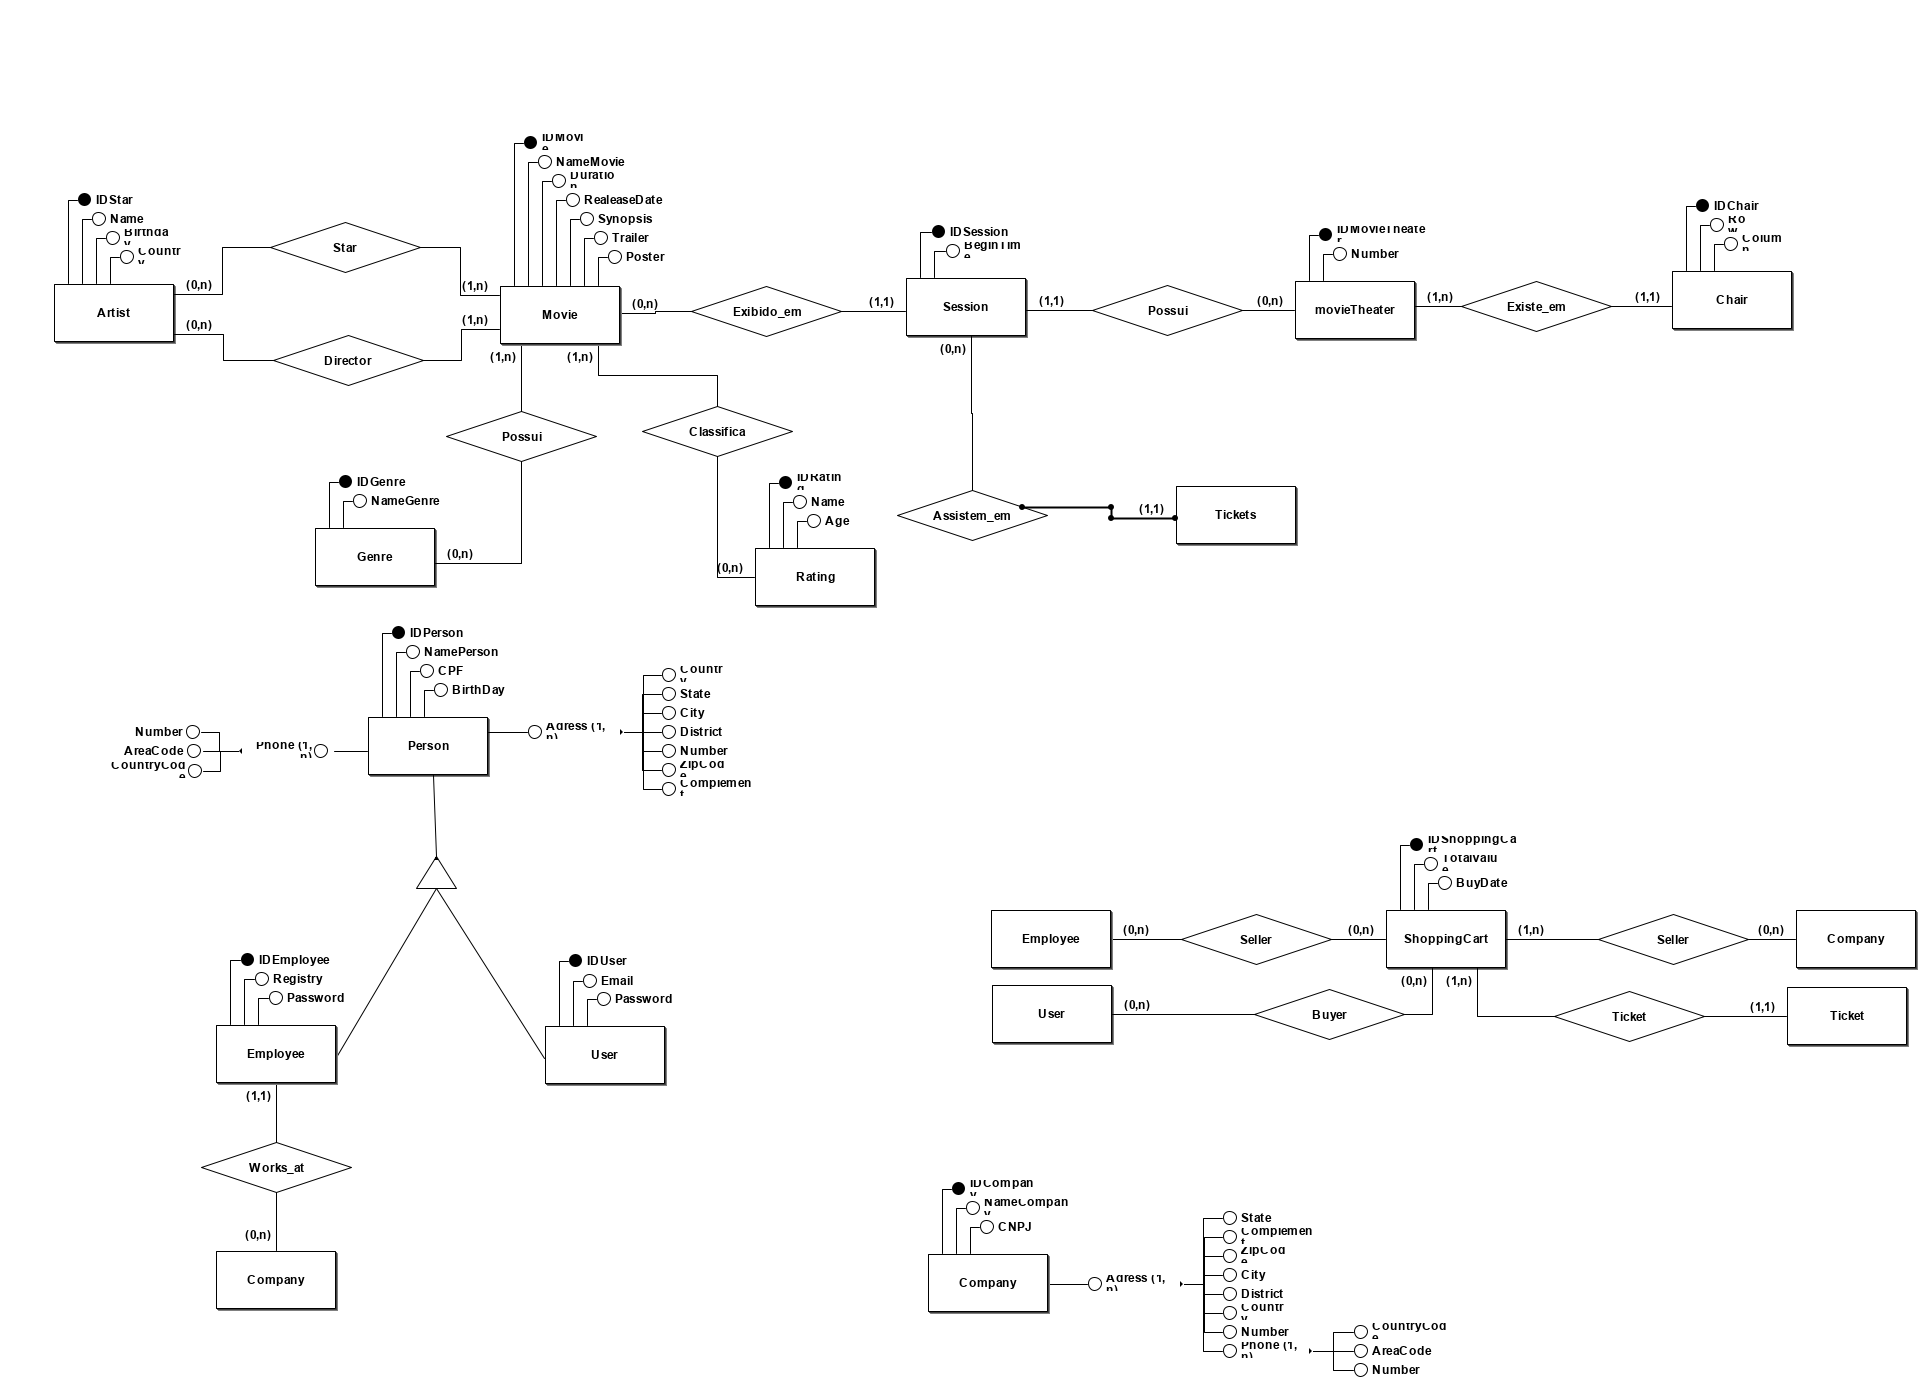
\includegraphics[width=\columnwidth]{UnBCineFlix_MER}%
\caption{Modelo Entidade Relacionamento}%
\label{fig:mer}%
\end{figure}

\section{Modelo Relacional}

Na figura \ref{fig:mr} mostramos o modelo relacional utilizado para implementação  do programa

\begin{figure}[h]
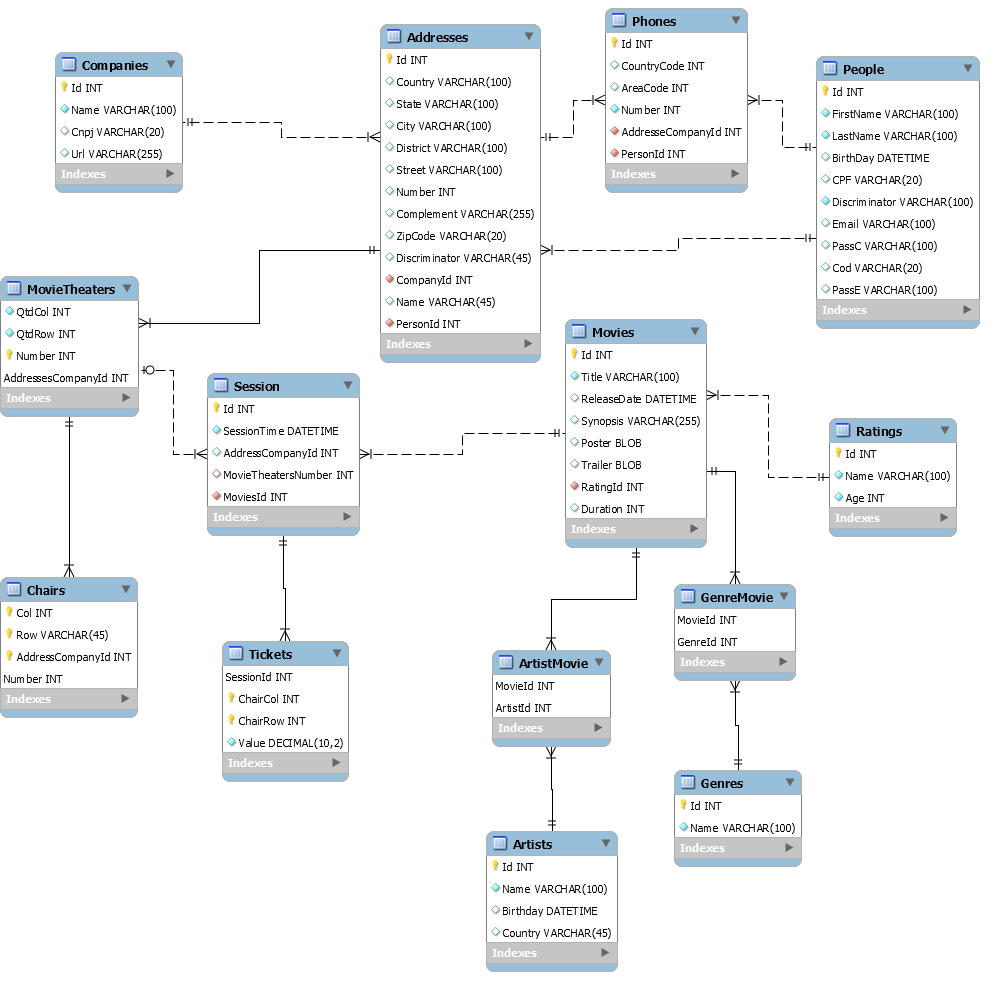
\includegraphics[width=\columnwidth]{UnBCineFlix_MR}%
\caption{Modelo Relacional}%
\label{fig:mr}%
\end{figure}

\section{Consultas}

Nesta seção mostramos exemplo de consultas que podem ser realizadas nesse modelo relacional de banco de dados.

\begin{lstlisting}
		use unbcineflix;
		
		select * FROM movies, ratings, genremovies, genres where ratingid = ratings.id and movies.id = genremovies.movieid and genremovies.genreid = genres.id;
		
		select * from movies, artistmovies, artists where Movies.id = artistmovies.MovieId and artistmovies.ArtistId = artists.Id;
		
		select * from movietheaters, addresses,companies where addresses.Id = movietheaters.AddressCompanyId and addresses.CompanyId = companies.Id and addresses.Discriminator = 'AddressCompany';
		
		select * from session, movietheaters, tickets where session.Id = tickets.SessionId and session.AddressCompanyId = movietheaters.AddressCompanyId and movietheaters.MovieTheaterNumber = session.MovieTheaterNumber;
		
		select * from people, addresses,phones where people.id = addresses.PersonId and people.id = phones.PersonId and addresses.Discriminator = 'AddressPerson';
\end{lstlisting}

\section{Álgebra Relacional}

Nesta seção mostramos as consulta acima realizadas, mas em álgebra relacional.

\begin{eqnarray*}
\sigma_{\textrm{Movies.RatingId = Ratings.Id and Movies.Id = GenreMovies.MovieId and genremovies.genreid = genres.id }}\\
(\textrm{Movies} \times \textrm{Ratings} \times \textrm{GenreMovies} \times \textrm{Genre})
\end{eqnarray*}

\begin{eqnarray*}
\sigma_{\textrm{Movies.id = artistmovies.MovieId and artistmovies.ArtistId = artists.Id}}\\
( \textrm{ movies} \times  \textrm{artistmovies} \times{ artists} )
\end{eqnarray*}


\begin{eqnarray*}
\sigma_{\textrm{addresses.Id = movietheaters.AddressCompanyId and addresses.CompanyId = companies.Id}}\\
_{\textrm{ and addresses.Discriminator = `AddressCompany'}}\\
(\textrm{movietheaters} \times \textrm{addresses} \times \textrm{companies})
\end{eqnarray*}

\begin{eqnarray*}
\sigma_{\textrm{session.Id = tickets.SessionId and session.AddressCompanyId = movietheaters.AddressCompanyId}}\\
_{ \textrm{and movietheaters.MovieTheaterNumber = session.MovieTheaterNumber}}\\
(\textrm{session} \times \textrm{ movietheaters} \times \textrm{ tickets})\\
\end{eqnarray*}

\begin{eqnarray}
\sigma_{ \textrm{people.id = addresses.PersonId and people.id = phones.PersonId and addresses.Discriminator = 'AddressPerson'}}\\
(people, addresses,phones)
\end{eqnarray}

\section{Views}

Nesta parte mostramos exemplos da utilização de Views no código do SQL.

\begin{lstlisting}
		use unbcineflix;

		drop view addresscompany;

		drop view AddressPerson;

		drop view SoldTickets;

		create view AddressCompany as SELECT Country,state, city, Street, number, zipcode, name from addresses WHERE addresses.Discriminator = 'AddressCompany';

		create view AddressPerson as SELECT Country,state, city, Street, number, zipcode from addresses WHERE addresses.Discriminator = 'AddressPerson';

		create view SoldTickets as select session.id as 'numero sessao', movies.Title as 'Titulo do filme', session.MovieTheaterNumber as 'sala', session.SessionTime as 'dia e hora', ChairCol as 'numero coluna', ChairRow  as 'numero fileira', Value as 'valor' from session, movietheaters, tickets, movies where session.Id = tickets.SessionId and session.AddressCompanyId = movietheaters.AddressCompanyId and movietheaters.MovieTheaterNumber = session.MovieTheaterNumber and session.MovieId = movies.id;

		select * from addresscompany;

		select * from AddressPerson;

		select * from SoldTickets;
\end{lstlisting}

Na figura \ref{fig:view_soldticket} podemos ver um exemplo de resultado mostrado pela viu SoldTickets.

\begin{figure}%
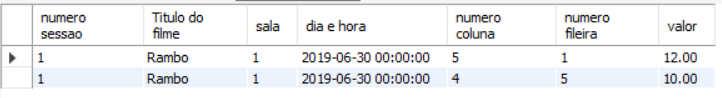
\includegraphics[width=\columnwidth]{View_exemplo}%
\caption{Exemplo de resultado da View SoldTickets}%
\label{fig:view_soldticket}%
\end{figure}

\section{Script Sql}

Nesta seção mostramos o script sql para geração do banco de dados, que foi gerado utilizando o modelo acima e foi gerado automaticamente pelo MySQL.

\begin{lstlisting}
		-- MySQL Script generated by MySQL Workbench
		-- Thu Jun 27 18:36:45 2019
		-- Model: New Model    Version: 2.0
		-- MySQL Workbench Forward Engineering

		SET @OLD_UNIQUE_CHECKS=@@UNIQUE_CHECKS, UNIQUE_CHECKS=0;
		SET @OLD_FOREIGN_KEY_CHECKS=@@FOREIGN_KEY_CHECKS, FOREIGN_KEY_CHECKS=0;
		SET @OLD_SQL_MODE=@@SQL_MODE, SQL_MODE='ONLY_FULL_GROUP_BY,STRICT_TRANS_TABLES,NO_ZERO_IN_DATE,NO_ZERO_DATE,ERROR_FOR_DIVISION_BY_ZERO,NO_ENGINE_SUBSTITUTION';

		-- -----------------------------------------------------
		-- Schema UnBCineFlix
		-- -----------------------------------------------------
		DROP SCHEMA IF EXISTS `UnBCineFlix` ;

		-- -----------------------------------------------------
		-- Schema UnBCineFlix
		-- -----------------------------------------------------
		CREATE SCHEMA IF NOT EXISTS `UnBCineFlix` DEFAULT CHARACTER SET utf8 ;
		USE `UnBCineFlix` ;

		-- -----------------------------------------------------
		-- Table `UnBCineFlix`.`Addresses`
		-- -----------------------------------------------------
		CREATE TABLE IF NOT EXISTS `UnBCineFlix`.`Addresses` (
			`Id` INT NOT NULL AUTO_INCREMENT,
			`Country` VARCHAR(100) NULL,
			`State` VARCHAR(100) NULL,
			`City` VARCHAR(100) NULL,
			`District` VARCHAR(100) NULL,
			`Street` VARCHAR(100) NULL,
			`Number` INT NULL,
			`Complement` VARCHAR(255) NULL,
			`ZipCode` VARCHAR(20) NULL,
			`Discriminator` VARCHAR(45) NULL,
			`CompanyId` INT NOT NULL,
			`Name` VARCHAR(45) NULL,
			`PersonId` INT NOT NULL,
			PRIMARY KEY (`Id`),
			INDEX `fk_Addresses_People1_idx` (`PersonId` ASC) VISIBLE,
			INDEX `fk_Addresses_Companies1_idx` (`CompanyId` ASC) VISIBLE,
			CONSTRAINT `fk_Addresses_People1`
				FOREIGN KEY (`PersonId`)
				REFERENCES `UnBCineFlix`.`People` (`Id`)
				ON DELETE NO ACTION
				ON UPDATE NO ACTION,
			CONSTRAINT `fk_Addresses_Companies1`
				FOREIGN KEY (`CompanyId`)
				REFERENCES `UnBCineFlix`.`Companies` (`Id`)
				ON DELETE NO ACTION
				ON UPDATE NO ACTION)
		ENGINE = InnoDB;


		-- -----------------------------------------------------
		-- Table `UnBCineFlix`.`ArtistMovie`
		-- -----------------------------------------------------
		CREATE TABLE IF NOT EXISTS `UnBCineFlix`.`ArtistMovie` (
			`MovieId` INT NOT NULL,
			`ArtistId` INT NOT NULL,
			PRIMARY KEY (`MovieId`, `ArtistId`),
			INDEX `fk_Movie_has_Artist_Artist1_idx` (`ArtistId` ASC) VISIBLE,
			INDEX `fk_Movie_has_Artist_Movie1_idx` (`MovieId` ASC) VISIBLE,
			CONSTRAINT `fk_Movie_has_Artist_Movie1`
				FOREIGN KEY (`MovieId`)
				REFERENCES `UnBCineFlix`.`Movies` (`Id`)
				ON DELETE NO ACTION
				ON UPDATE NO ACTION,
			CONSTRAINT `fk_Movie_has_Artist_Artist1`
				FOREIGN KEY (`ArtistId`)
				REFERENCES `UnBCineFlix`.`Artists` (`Id`)
				ON DELETE NO ACTION
				ON UPDATE NO ACTION)
		ENGINE = InnoDB;


		-- -----------------------------------------------------
		-- Table `UnBCineFlix`.`Artists`
		-- -----------------------------------------------------
		CREATE TABLE IF NOT EXISTS `UnBCineFlix`.`Artists` (
			`Id` INT NOT NULL,
			`Name` VARCHAR(100) NOT NULL,
			`Birthday` DATETIME NULL,
			`Country` VARCHAR(45) NULL,
			PRIMARY KEY (`Id`))
		ENGINE = InnoDB;


		-- -----------------------------------------------------
		-- Table `UnBCineFlix`.`Chairs`
		-- -----------------------------------------------------
		CREATE TABLE IF NOT EXISTS `UnBCineFlix`.`Chairs` (
			`Col` INT NOT NULL,
			`Row` VARCHAR(45) NOT NULL,
			`AddressCompanyId` INT NOT NULL,
			`Number` INT NOT NULL,
			PRIMARY KEY (`Col`, `Row`, `AddressCompanyId`, `Number`),
			INDEX `fk_Chairs_MovieTheaters1_idx` (`AddressCompanyId` ASC, `Number` ASC) VISIBLE,
			CONSTRAINT `fk_Chairs_MovieTheaters1`
				FOREIGN KEY (`Number`)
				REFERENCES `UnBCineFlix`.`MovieTheaters` (`Number`)
				ON DELETE NO ACTION
				ON UPDATE NO ACTION)
		ENGINE = InnoDB;


		-- -----------------------------------------------------
		-- Table `UnBCineFlix`.`Companies`
		-- -----------------------------------------------------
		CREATE TABLE IF NOT EXISTS `UnBCineFlix`.`Companies` (
			`Id` INT NOT NULL AUTO_INCREMENT,
			`Name` VARCHAR(100) NOT NULL,
			`Cnpj` VARCHAR(20) NULL,
			`Url` VARCHAR(255) NULL,
			PRIMARY KEY (`Id`))
		ENGINE = InnoDB;


		-- -----------------------------------------------------
		-- Table `UnBCineFlix`.`GenreMovie`
		-- -----------------------------------------------------
		CREATE TABLE IF NOT EXISTS `UnBCineFlix`.`GenreMovie` (
			`MovieId` INT NOT NULL,
			`GenreId` INT ZEROFILL NOT NULL,
			PRIMARY KEY (`MovieId`, `GenreId`),
			INDEX `fk_Movie_has_Genre_Genre1_idx` (`GenreId` ASC) VISIBLE,
			INDEX `fk_Movie_has_Genre_Movie1_idx` (`MovieId` ASC) VISIBLE,
			CONSTRAINT `fk_Movie_has_Genre_Movie1`
				FOREIGN KEY (`MovieId`)
				REFERENCES `UnBCineFlix`.`Movies` (`Id`)
				ON DELETE NO ACTION
				ON UPDATE NO ACTION,
			CONSTRAINT `fk_Movie_has_Genre_Genre1`
				FOREIGN KEY (`GenreId`)
				REFERENCES `UnBCineFlix`.`Genres` (`Id`)
				ON DELETE NO ACTION
				ON UPDATE NO ACTION)
		ENGINE = InnoDB;


		-- -----------------------------------------------------
		-- Table `UnBCineFlix`.`Genres`
		-- -----------------------------------------------------
		CREATE TABLE IF NOT EXISTS `UnBCineFlix`.`Genres` (
			`Id` INT ZEROFILL NOT NULL,
			`Name` VARCHAR(100) NOT NULL,
			PRIMARY KEY (`Id`))
		ENGINE = InnoDB;


		-- -----------------------------------------------------
		-- Table `UnBCineFlix`.`MovieTheaters`
		-- -----------------------------------------------------
		CREATE TABLE IF NOT EXISTS `UnBCineFlix`.`MovieTheaters` (
			`QtdCol` INT NOT NULL,
			`QtdRow` INT NOT NULL,
			`Number` INT NOT NULL,
			`AddressesCompanyId` INT NOT NULL,
			PRIMARY KEY (`Number`, `AddressesCompanyId`),
			INDEX `fk_MovieTheaters_Addresses1_idx` (`AddressesCompanyId` ASC) VISIBLE,
			CONSTRAINT `fk_MovieTheaters_Addresses1`
				FOREIGN KEY (`AddressesCompanyId`)
				REFERENCES `UnBCineFlix`.`Addresses` (`Id`)
				ON DELETE NO ACTION
				ON UPDATE NO ACTION)
		ENGINE = InnoDB;


		-- -----------------------------------------------------
		-- Table `UnBCineFlix`.`Movies`
		-- -----------------------------------------------------
		CREATE TABLE IF NOT EXISTS `UnBCineFlix`.`Movies` (
			`Id` INT NOT NULL AUTO_INCREMENT,
			`Title` VARCHAR(100) NOT NULL,
			`ReleaseDate` DATETIME NULL,
			`Synopsis` VARCHAR(255) NULL,
			`Poster` BLOB NULL,
			`Trailer` BLOB NULL,
			`RatingId` INT NOT NULL,
			`Duration` INT NULL,
			PRIMARY KEY (`Id`),
			INDEX `fk_Movie_Rating1_idx` (`RatingId` ASC) VISIBLE,
			CONSTRAINT `fk_Movie_Rating1`
				FOREIGN KEY (`RatingId`)
				REFERENCES `UnBCineFlix`.`Ratings` (`Id`)
				ON DELETE NO ACTION
				ON UPDATE NO ACTION)
		ENGINE = InnoDB;


		-- -----------------------------------------------------
		-- Table `UnBCineFlix`.`People`
		-- -----------------------------------------------------
		CREATE TABLE IF NOT EXISTS `UnBCineFlix`.`People` (
			`Id` INT NOT NULL AUTO_INCREMENT,
			`FirstName` VARCHAR(100) NOT NULL,
			`LastName` VARCHAR(100) NOT NULL,
			`BirthDay` DATETIME NULL,
			`CPF` VARCHAR(20) NULL,
			`Discriminator` VARCHAR(100) NOT NULL,
			`Email` VARCHAR(100) NULL,
			`PassC` VARCHAR(100) NULL,
			`Cod` VARCHAR(20) NULL,
			`PassE` VARCHAR(100) NULL,
			PRIMARY KEY (`Id`))
		ENGINE = InnoDB;


		-- -----------------------------------------------------
		-- Table `UnBCineFlix`.`Phones`
		-- -----------------------------------------------------
		CREATE TABLE IF NOT EXISTS `UnBCineFlix`.`Phones` (
			`Id` INT NOT NULL AUTO_INCREMENT,
			`CountryCode` INT NULL,
			`AreaCode` INT NULL,
			`Number` INT NOT NULL,
			`AddresseCompanyId` INT NOT NULL,
			`PersonId` INT NOT NULL,
			PRIMARY KEY (`Id`),
			INDEX `fk_Phones_Addresses1_idx` (`AddresseCompanyId` ASC) VISIBLE,
			INDEX `fk_Phones_People1_idx` (`PersonId` ASC) VISIBLE,
			CONSTRAINT `fk_Phones_Addresses1`
				FOREIGN KEY (`AddresseCompanyId`)
				REFERENCES `UnBCineFlix`.`Addresses` (`Id`)
				ON DELETE NO ACTION
				ON UPDATE NO ACTION,
			CONSTRAINT `fk_Phones_People1`
				FOREIGN KEY (`PersonId`)
				REFERENCES `UnBCineFlix`.`People` (`Id`)
				ON DELETE NO ACTION
				ON UPDATE NO ACTION)
		ENGINE = InnoDB;


		-- -----------------------------------------------------
		-- Table `UnBCineFlix`.`Ratings`
		-- -----------------------------------------------------
		CREATE TABLE IF NOT EXISTS `UnBCineFlix`.`Ratings` (
			`Id` INT NOT NULL AUTO_INCREMENT,
			`Name` VARCHAR(100) NOT NULL,
			`Age` INT NOT NULL,
			PRIMARY KEY (`Id`))
		ENGINE = InnoDB;


		-- -----------------------------------------------------
		-- Table `UnBCineFlix`.`Session`
		-- -----------------------------------------------------
		CREATE TABLE IF NOT EXISTS `UnBCineFlix`.`Session` (
			`Id` INT NOT NULL AUTO_INCREMENT,
			`SessionTime` DATETIME NOT NULL,
			`AddressCompanyId` INT NULL,
			`MovieTheatersNumber` INT NULL,
			`MoviesId` INT NOT NULL,
			PRIMARY KEY (`Id`),
			INDEX `fk_Session_MovieTheaters1_idx` (`AddressCompanyId` ASC, `MovieTheatersNumber` ASC) VISIBLE,
			INDEX `fk_Session_Movies1_idx` (`MoviesId` ASC) VISIBLE,
			CONSTRAINT `fk_Session_MovieTheaters1`
				FOREIGN KEY (`MovieTheatersNumber`)
				REFERENCES `UnBCineFlix`.`MovieTheaters` (`Number`)
				ON DELETE NO ACTION
				ON UPDATE NO ACTION,
			CONSTRAINT `fk_Session_Movies1`
				FOREIGN KEY (`MoviesId`)
				REFERENCES `UnBCineFlix`.`Movies` (`Id`)
				ON DELETE NO ACTION
				ON UPDATE NO ACTION)
		ENGINE = InnoDB;


		-- -----------------------------------------------------
		-- Table `UnBCineFlix`.`Tickets`
		-- -----------------------------------------------------
		CREATE TABLE IF NOT EXISTS `UnBCineFlix`.`Tickets` (
			`SessionId` INT NOT NULL,
			`ChairCol` INT NOT NULL,
			`ChairRow` INT NOT NULL,
			`Value` DECIMAL(10,2) NOT NULL,
			PRIMARY KEY (`SessionId`, `ChairCol`, `ChairRow`),
			INDEX `fk_Tickets_Session1_idx` (`SessionId` ASC) VISIBLE,
			CONSTRAINT `fk_Tickets_Session1`
				FOREIGN KEY (`SessionId`)
				REFERENCES `UnBCineFlix`.`Session` (`Id`)
				ON DELETE NO ACTION
				ON UPDATE NO ACTION)
		ENGINE = InnoDB;


		SET SQL_MODE=@OLD_SQL_MODE;
		SET FOREIGN_KEY_CHECKS=@OLD_FOREIGN_KEY_CHECKS;
		SET UNIQUE_CHECKS=@OLD_UNIQUE_CHECKS;
\end{lstlisting}


\section{Camada de Persistência}

Para acesso ao banco de Dados foi utilizado o Entity FrameWork Core versão 2.2.4 e o sistema MySQL como banco de dados de persistência, a seguir mostramos o código de persistência da aplicação e exemplos do controlador de acesso. 

O código a seguir é o código de ``Context'' do EntityFramework Core o qual foi desenvolvido seguindo os padrão do nomeclatura e de desenvolvimento exigidos pela comunidade, utilizamos esse FrameWork devido a sua camada de middleware que faz a conversão automática do sistema relacional para a orientação objeto utilizado no programa que foi desenvolvido com C\# e ASP.NET Core 2.2 tendo como objetivo final uma aplicação Web que poudesse ser executada por um usuario domestico ou pelos adiministradores do sistema diretamente da empresa, sendo assim uma aplicação completa para uma empresa. 

\lstset{style=cstyle} 

\begin{lstlisting}
using Microsoft.EntityFrameworkCore;
using System;
using System.Collections.Generic;
using System.Text.RegularExpressions;
using UnBCineFlix.Models;

namespace UnBCineFlix.DAL
{
		public class UnBCineFlixContext : DbContext
		{
				public DbSet<Address> Addresses { get; set; }
				public DbSet<AddressCompany> AddressCompanies { get; set; }
				public DbSet<AddressPerson> AddressPeople { get; set; }
				public DbSet<Artist> Artists { get; set; }
				public DbSet<ArtistMovie> ArtistMovies { get; set; }
				public DbSet<Chair> Chairs { get; set; }
				public DbSet<Company> Companies { get; set; }
				public DbSet<Customer> Customers { get; set; }
				public DbSet<Employee> Employees { get; set; }
				//errorviemodel
				public DbSet<Genre> Genres { get; set; }
				public DbSet<GenreMovie> GenreMovies { get; set; }
				public DbSet<Movie> Movies { get; set; }
				public DbSet<MovieTheater> MovieTheaters { get; set; }
				public DbSet<Person> People { get; set; }
				public DbSet<Phone> Phones { get; set; }
				public DbSet<Rating> Ratings { get; set; }
				public DbSet<Session> Session { get; set; }
				public DbSet<Ticket> Tickets { get; set; }

				public UnBCineFlixContext()
				{
				}
				public UnBCineFlixContext(DbContextOptions<UnBCineFlixContext> option)
		: base(option)
				{
				}
				protected override void OnModelCreating(ModelBuilder modelBuilder)
				{
						//Primary Key setup space
						#region pk
						modelBuilder.Entity<Address>().HasKey(a => a.Id);
						modelBuilder.Entity<Person>().HasKey(p => p.Id);
						modelBuilder.Entity<Phone>().HasKey(ph => ph.Id);
						modelBuilder.Entity<Rating>().HasKey(r => r.Id);
						modelBuilder.Entity<Artist>().HasKey(ar => ar.Id);
						modelBuilder.Entity<Movie>().HasKey(m => m.Id);
						modelBuilder.Entity<Company>().HasKey(c => c.Id);
						modelBuilder.Entity<Session>().HasKey(s => s.Id);
						modelBuilder.Entity<ArtistMovie>().HasKey(am => new { am.MovieId, am.ArtistId });
						modelBuilder.Entity<GenreMovie>().HasKey(gm => new { gm.GenreId, gm.MovieId });
						modelBuilder.Entity<MovieTheater>().HasKey(mt => new { mt.AddressCompanyId, mt.MovieTheaterNumber });
						modelBuilder.Entity<Chair>().HasKey(ch => new { ch.AddressCompanyId, ch.MovieTheaterNumber, ch.Row, ch.Col });
						modelBuilder.Entity<Ticket>().HasKey(t => new { t.SessionId, t.ChairRow, t.ChairCol });
						#endregion

						//foreign key setup space
						#region fk
						modelBuilder.Entity<AddressPerson>().HasOne(a => a.Person).WithMany(p => p.Addresses).HasForeignKey(a => a.PersonId).OnDelete(DeleteBehavior.Cascade);
						modelBuilder.Entity<Phone>().HasOne(ph => ph.Person).WithMany(p => p.Phones).HasForeignKey(p => p.PersonId).OnDelete(DeleteBehavior.Cascade);

						modelBuilder.Entity<AddressCompany>().HasOne(a => a.Company).WithMany(c => c.Addresses).HasForeignKey(ac => ac.CompanyId).OnDelete(DeleteBehavior.Cascade);
						modelBuilder.Entity<Phone>().HasOne(ph => ph.AddressCompany).WithMany(c => c.Phones).HasForeignKey(p => p.AddressCompanyId).OnDelete(DeleteBehavior.Cascade);

						modelBuilder.Entity<ArtistMovie>().HasOne(am => am.Artist).WithMany(a => a.Movies).HasForeignKey(am => am.ArtistId).OnDelete(DeleteBehavior.Cascade);
						modelBuilder.Entity<ArtistMovie>().HasOne(am => am.Movie).WithMany(m => m.Artists).HasForeignKey(am => am.MovieId).OnDelete(DeleteBehavior.Cascade);

						modelBuilder.Entity<GenreMovie>().HasOne(gm => gm.Genre).WithMany(g => g.GenreMovies).HasForeignKey(gm => gm.GenreId).IsRequired();
						modelBuilder.Entity<GenreMovie>().HasOne(gm => gm.Movie).WithMany(m => m.GenreMovies).HasForeignKey(gm => gm.MovieId).IsRequired();

						modelBuilder.Entity<Movie>().HasOne(m => m.Rating).WithMany(r => r.Movies).HasForeignKey(m => m.RatingId).OnDelete(DeleteBehavior.SetNull);

						modelBuilder.Entity<MovieTheater>().HasOne(mt => mt.AddressCompany).WithMany(ac => ac.MovieTheaters).HasForeignKey(mt => mt.AddressCompanyId);

						modelBuilder.Entity<Chair>().HasOne(ch => ch.MovieTheater).WithMany(mt => mt.Chairs).HasForeignKey(ch => new { ch.AddressCompanyId, ch.MovieTheaterNumber }).IsRequired().OnDelete(DeleteBehavior.Cascade);

						modelBuilder.Entity<Session>().HasOne(s => s.MovieTheater).WithMany(mt => mt.Sessions).HasForeignKey(s => new { s.AddressCompanyId, s.MovieTheaterNumber });
						modelBuilder.Entity<Session>().HasOne(s => s.Movie).WithMany(m => m.Sessions).HasForeignKey(s => s.MovieId);

						modelBuilder.Entity<Ticket>().HasOne(t => t.Session).WithMany(s => s.Tickets).HasForeignKey(t=> t.SessionId).IsRequired();
						#endregion

						//Espaco para propriedades
						#region properties
						modelBuilder.Entity<MovieTheater>().Property<int>("QtdRow").IsRequired();
						modelBuilder.Entity<MovieTheater>().Property<int>("QtdCol").IsRequired();
						#endregion

						//Heranca
						#region heritage
						modelBuilder.Entity<Customer>().HasBaseType<Person>();
						modelBuilder.Entity<Employee>().HasBaseType<Person>();

						modelBuilder.Entity<AddressCompany>(ac => { ac.HasBaseType<Address>(); });
						modelBuilder.Entity<AddressPerson>(ac => { ac.HasBaseType<Address>(); });
						#endregion

						//Seeding the DataBase
						#region seed
						modelBuilder.Entity<Company>().HasData(
								new Company { Id = 1, Name = "Cine Marx" }
						);

						modelBuilder.Entity<AddressCompany>().HasData(
								new AddressCompany { Id = 1, CompanyId = 1, City = "brasilia", District = "Asa Sul", Street = "sql", Number = 42, Complement = null, Country = "Brasil", State = "DF", ZipCode = 7000000, Name = "Brasilia Park"}
						);

						modelBuilder.Entity<MovieTheater>().HasData(
								new MovieTheater (qtdCol:10, qtdRow:10){ MovieTheaterNumber = 1, AddressCompanyId = 1}
						);

						// inicializa as cadeira da sala->todas.
						for (int i = 0; i < 10; i++)
						{
								for (int j = 0; j < 10; j++)
								{
										var c = new Chair(i, j);
										c.AddressCompanyId = 1;
										c.MovieTheaterNumber = 1;
										modelBuilder.Entity<Chair>().HasData(c);
								}
						}
						modelBuilder.Entity<Customer>().HasData(
								new Customer { Id = 1, FirstName = "Dovakin", LastName = "Alcantara", BirthDay = new DateTime(1911, 11, 11), CPF = "000.000.000-00", Email = "email@email", PassC = "muito louco" },
								new Customer { Id = 2, FirstName = "Machado", LastName = "de assis", BirthDay = new DateTime(1911, 11, 11), CPF = "333.333.333-33", Email = "email@email", PassC = "muito louco 2" }
						);

						modelBuilder.Entity<Employee>().HasData(
								new Employee { Id = 3, FirstName = "Dovakin", LastName = "Alcantara", BirthDay = new DateTime(1911, 11, 11), CPF = "000.000.000-00", Cod = 123456, PassE = "12" }
						);

						modelBuilder.Entity<AddressPerson>().HasData(
								new AddressPerson { Id = 3, City = "brasilia", District = "Asa Sul", Street = "sql", Number = 42, Complement = null, Country = "Brasil", State = "DF", ZipCode = 7000000, PersonId = 1 },
								new AddressPerson { Id = 2, City = "brasilia", District = "Asa norte", Street = "Campus Darcy Ribeiro", Number = 0, Complement = "ICC Norte", Country = "Brasil", State = "DF", ZipCode = 70000000, PersonId = 2 }
						);

						modelBuilder.Entity<Phone>().HasData(
								new Phone { Id = 1, CountryCode = 55, AreaCode = 61, Number = 55551234, PersonId = 1 },
								new Phone { Id = 2, CountryCode = 55, AreaCode = 61, Number = 999954321, AddressCompanyId = 1 },
								new Phone { Id = 3, CountryCode = 55, AreaCode = 61, Number = 999912345, PersonId = 2 }
						);

						modelBuilder.Entity<Rating>().HasData(
								new Rating { Id = 1, Name = "Livre", Age = 0 },
								new Rating { Id = 2, Name = "NR 10", Age = 10 },
								new Rating { Id = 3, Name = "NR 12", Age = 12 },
								new Rating { Id = 4, Name = "NR 14", Age = 14 },
								new Rating { Id = 5, Name = "NR 16", Age = 16 },
								new Rating { Id = 6, Name = "NR 18", Age = 18 }
						);

						modelBuilder.Entity<Artist>().HasData(
								new Artist { Id = 1, Name = "Silvester Stallone", Country = "USA", BirthDay = new DateTime(1946, 6, 6) },
								new Artist { Id = 2, Name = "Arnold Schwarzenegger", Country = "Autria", BirthDay = new DateTime(1947, 6, 30) }
						);
						modelBuilder.Entity<Movie>().HasData(
								new Movie { Id = 1, Title = "Rambo 3", Duration = 180, ReleaseDate = new DateTime(2000, 12, 25), RatingId = 6 },
								new Movie { Id = 2, Title = "Rambo 2", Duration = 200, ReleaseDate = new DateTime(1990, 12, 25), RatingId = 6 },
								new Movie { Id = 3, Title = "Rambo  ", Duration = 160, ReleaseDate = new DateTime(1985, 12, 25) }
						);

						modelBuilder.Entity<ArtistMovie>().HasData(
								new ArtistMovie { MovieId = 1, ArtistId = 1 },
								new ArtistMovie { MovieId = 2, ArtistId = 1 },
								new ArtistMovie { MovieId = 3, ArtistId = 1 },
								new ArtistMovie { MovieId = 1, ArtistId = 2 }
								);

						modelBuilder.Entity<Genre>().HasData(
								new Genre { Id = 1, Name = "Action" },
								new Genre { Id = 2, Name = "comedy" }
						);
						modelBuilder.Entity<GenreMovie>().HasData(
								new GenreMovie { MovieId = 1, GenreId = 1 },
								new GenreMovie { MovieId = 2, GenreId = 1 },
								new GenreMovie { MovieId = 3, GenreId = 1 }
								);
						modelBuilder.Entity<Session>().HasData(
								new Session { AddressCompanyId = 1, SessionTime = DateTime.Today.AddDays(3), MovieId = 3, MovieTheaterNumber = 1 , Id = 1}
								);

						modelBuilder.Entity<Ticket>().HasData(
								new Ticket { SessionId = 1, ChairCol = 4, ChairRow = 5, Value = 10 }
								);
						#endregion
				}
				protected override void OnConfiguring(DbContextOptionsBuilder optionsBuilder)
				{
						if (!optionsBuilder.IsConfigured)
						{
								optionsBuilder.UseMySQL("Server=localhost;DataBase=unbcineflix;Uid=root;Pwd=@VTQpZGC8*qkj\$uu");
						}
				}
		}
}
\end{lstlisting}

A seguir mostramos alguns exemplos de códigoo de acesso ao bando de dados leitura e escrita usando o Entity FrameWork e explicamos como ele funciona.

\begin{lstlisting}
var session = await _context.Session
		.Include(s => s.Tickets)
		.Include(s => s.Movie)
		.Include(s => s.MovieTheater)
				.ThenInclude(mt => mt.Chairs)
		.Include(s => s.MovieTheater)
				.ThenInclude(mt => mt.AddressCompany)
				.ThenInclude(ac => ac.Company)
		.FirstOrDefaultAsync(m => m.Id == id);
\end{lstlisting}

Acima mostramos o processo de leitura de uma Session no Banco de Dados, no quel é realizado um Join com os objetos/tabelas Tickets, Movie, MovieTheater, Chairs, AddresCompany, Company, pois nesse caso em especial queriamos mostrar que uma determinada sessão $i$ seria exibida em um determinado dia, em um determinado local, por uma determinada empressa, além de precisarmos saber quais cadeiras existem dentro da sala na qual a sessão será exibida e quais ingressos já foram vendidos.

\begin{lstlisting}
var ticket = await _context.Tickets
		.FirstOrDefaultAsync(t=> 
			(t.SessionId == sessionId && 
				t.ChairRow == chairRow && 
				t.ChairCol == chairCol));
\end{lstlisting}

Neste caso é uma busca bem mais simples, simplesmente queremos saber se o Ticket de uma dada Session, com uma determinada cadeira coluna (ChairCol) e Fileira (ChairRow) existe, ou seja, foi vendido.

\begin{lstlisting}
[HttpPost]
[ValidateAntiForgeryToken]
public async Task<IActionResult> Create([Bind("Id,Name,BirthDay,Country")] Artist artist)
{
		if (ModelState.IsValid)
		{
				_context.Add(artist);
				await _context.SaveChangesAsync();
				return RedirectToAction(nameof(Index));
		}
		return View(artist);
}
\end{lstlisting}
Acima mostramos o método completo da camada de persistência, controlador, que é usado para adicionar um novo objeto artista dentro do banco de dados relacional, pela simplicidade proporcionada pelo framework utilizado acreditamos ser desnecessário separar a camada de persistência do controlador, apesar que seria especialmente útil se desejarmos 

\section{Avaliação das Formas Normais}

%\pagebreak
%\bibliographystyle{plain}
%\bibliography{MyLib} 
\end{document} 